\documentclass[11pt,psfig]{article}
\usepackage{epsfig}
\usepackage{times}
\usepackage{amssymb}
\usepackage{float}
\usepackage[T1]{fontenc}
\usepackage[utf8]{inputenc}
\usepackage{authblk}

\newcount\refno\refno=1
\def\ref{\the\refno \global\advance\refno by 1}
\def\ux{\underline{x}}
\def\uw{\underline{w}}
\def\bw{\underline{w}}
\def\ut{\underline{\theta}}
\def\umu{\underline{\mu}} 
\def\bmu{\underline{\mu}} 
\def\be{p_e^*}
\newcount\eqnumber\eqnumber=1
\def\eq{\the \eqnumber \global\advance\eqnumber by 1}
\def\eqs{\eq}
\def\eqn{\eqno(\eq)}

 \pagestyle{empty}
\def\baselinestretch{1.1}
\topmargin1in \headsep0.3in
\topmargin0in \oddsidemargin0in \textwidth6.5in \textheight8.5in
\begin{document}
\setlength{\parskip}{1.2ex plus0.3ex minus 0.3ex}


\thispagestyle{empty} \pagestyle{myheadings} \markright{G}



\title{A Greedy Heuristic using Redundancy for the Data Layout Problem}
%\author{Zachary DeStefano, Shan Jiang, Gopi Meenakshisundaram, Sung-Eui Yoon\\ University of California, Irvine}
\author[1]{Zachary DeStefano}
\author[1]{Shan Jiang}
\author[1]{Gopi Meenakshisundaram}
\author[2]{Sung-Eui Yoon}
\affil[1]{University of California, Irvine}
\affil[2]{KAIST}

\date{October 21, 2014}

\maketitle

\vfill\eject

\section*{Abstract}

In Computer Graphics, in order to compute an efficient cache oblivious mesh layout we must figure out the optimal method for laying out the data units. Finding a deterministic solution to the problem is NP-hard so various heuristics have been proposed. In this paper, we present a solution to the problem based on introducing redundancy to the layout. It will reduce seek time while using the least amount of redundancy possible. This will prove to be a better heuristic than existing ones proposed both analytically and experimentally. 

\section*{Introduction}

The Data Layout Problem can be formulated as follows. The input is a linear sequence of data units. Each of the data units is assigned at least one color and many of them have multiple colors assigned. The length of a color is the distance from its first data unit to its last data unit. The data units can be rearranged as desired. The output we would like is the sequence of data units that will minimize the total length of all the colors. \\
\\
In Yoon's paper \cite{cacheobliviouslayout}, the Data Layout Problem is described as well as the metric that is motivating the above definition. We noticed that access patterns described in the paper can be very general and there could easily be data units that are far apart in the sequence but need to be accessed together. This led us to realize that if we copy data units and move them closer to other ones that share the same access pattern then we could save a lot of seek time without adding much storage space. The rest of this paper is about the algorithm developed to optimize seek time while minimizing the redundancy required to accomplish that. 

\newpage

\section*{Related Work}

Massive model rendering has been a challenging field of research in computer graphics for decades. A large body of literature has been built on different aspects of solving this problem. Here we briefly discuss work in two main approaches in this topic, Out-Of-Core Rendering and Image-based Rendering. 

\subsection*{Out-Of-Core Rendering}

Large-scale model rendering generally implies that the geometry data is so large that one must employ a secondary storage device during rendering. Thus, due to the nature of secondary storage devices and the architecture of modern computers, data fetching and data management for main memory can become performance bottlenecks during rendering. To remove or reduce these bottlenecks, research on out-of-core rendering aims at fetching, caching, and managing data in efficient ways. Coorea et al \cite{iwalk} introduced the iWalk system, in which octree-based spatialization is applied on geometry data, and this allowed only visible data to be retrieved from hard drives. Varadhan et al \cite{outofcore} also focused on isolating data required by each frame, but in a graph-based algorithm. A scene graph is generated in level of details and frame-to-frame visibility consistence. Parallel processing is also employed so that rendering the active part of the scene and fetching objects from the disk are done simultaneously. Sajadi et al \cite{pagebased} improved efficiency of out-of-core rendering by preprocessing the data set into a form of disk pages. The disk pages are self-contained data units with fixed size. This method avoids data management on the primitive level which reduces the time complexity by orders of magnitude. By utilizing a globally optimized data layout, caching can be further improved. Globally optimized data layout is an NP hard problem. Nevertheless, Yoon et al \cite{cacheobliviouslayout} provided a feasible method to try to compute it. Similar to other problems where an optimal permutation needs to be computed, they developed a hierarchical algorithm with a heuristic based on edge spans to get an approximated solution quickly.

\subsection*{Image-Based Rendering}

Image-based rendering techniques reduce the geometry of a massive model to a view-independent mesh along with pre-rendered textures. The number of primitives to be rendered is much less than the original model. Therefore, both data transferring time and rendering time can be greatly saved. The major drawback of image-based rendering is the lack of geometry information. Zhang et al \cite{imagebasedrendering} presented a survey of image-based rendering techniques. These techniques involve sampling the space using a plenoptic function in the first stage and then rendering the continuous plenoptic function in the next stage. It is similar to the technique in signal processing of sampling a set of numbers and then using those samples to get the continuous function and reconstructing the continuous function. The paper goes into detail on various applications of these techniques. Li et al \cite{compressionimagebased} explored various compression methods for image-based rendering. Specifically, they explored the benefits of three compression algorithms. All three proved to be able to achieve real time rendering of large models and they vary in the complexity of the decoding and the compression ratio they are able to achieve. 

\subsection*{Seek Time and Redundancy-based solutions}

In real time rendering, time spent on one frame can be roughly divided into data fetching time, online processing time, and rendering time. Data fetching time can be further decomposed into seek time and data transfer time. Sajadi et al \cite{ssdpaper} explored the reasons for the performance advantage of Solid-State Drives (SSD) over Hard-Disk Drives (HDD). The result shows clearly constant seek time of SSDs is the major reason that fetching data on SSDs is generally faster and more consistent than HDDs. Jiang et al \cite{singleseeklayout} minimized disk seeks to one or less for each frame by storing multiple copies of same data at different locations of secondary storage devices. These extra copies will be referred to as redundancy. The paper successfully showed that limited seeks lead to improvement of performance. However, to keep number of seeks being one or less, a large amount of redundancy is necessary, which is not practical for many applications. Jiang et al \cite{optimizingredundancy} generalized this approach by relaxing the number of seeks to a small threshold. This threshold is determined by time budget of each frame. In this way, the number of seeks required is relaxed to minimize amount of redundancy. This optimization is done through integer linear programming. This approach ended up reducing the amount of redundancy significantly. The algorithm however does not take data layout into account and is thus not an optimal solution. 

\newpage

\section*{Greedy Redundancy-based Cache Oblivious Mesh Layout Algorithm}

The main time when this problem arises is when walking through a large 3D environment. Since we cannot put all the geometric data into memory all at once, we want to make sure that as little time as possible is spent seeking out the new data units during walkthrough. Thus, we need to put the data units as close together as they can be. \\
\\
The algorithm in Yoon et al. computes a locally optimal solution. Our algorithm is meant to take over after a locally optimal solution has been found or approximated. The basic idea of the algorithm is to take data units and copy them to a place that reduces seek time. This way if a data unit should be in more than one place to optimize seek time then it will be. If the old data units end up not being used then we delete them. Because there are cases where we would delete old units, the first loop in the algorithm is to take care of those cases first as it would reduce seek time without adding any redundancy. In order to get this algorithm to work, there are a few important issues to consider. We need to know which data units should be copied, where it should be copied to, which data units should be used by each access requirement, and which how many data units should be copied. 

\subsection*{Which data unit}

Since we only care about the length of each access requirement, we will only be copying the data units that are on the endpoints of an access requirement. The key to this algorithm is that we are shortening each access requirement at each step, so hopefully we can get to a point where they are all grouped together. 

\subsection*{Where to locate data unit}

We want to copy the data units to somewhere between the one after the first one and the last one. That way we are guaranteed to reduce the seek time for the access requirement we care about. For our own access requirement, it won't matter where in that interval we place our data unit. However, for the other access requirements, we are adding one unit of seek time since that data unit gets inserted. Therefore, we want to find which place will interrupt the least number of access requirements. We then have to search through each unit to see where the least number of overlaps occurs. We can assume that we have already precomputed the number of overlaps at each unit. We now have a problem of given a dynamic set of intervals (access requirement ranges in our case), and an arbitrary range, what is the least number of overlapping intervals in that range?\\
\\
This problem is just find the least number in an arbitrary range. For our purposes, we will do a linear search through each entry in the range in order to find the ideal entry. If $k$ is the size of the access requirement, then this gives us $O(k)$ query time. Updates will also be $O(k)$ and construction will be $O(N)$ with N being the number of data units. There are other approaches, such as a range tree or dynamic programming, that may produce better query times, but their construction and update times will be worse as well as their storage. \\
\\
With dynamic programming, we would have to maintain a matrix where an entry $(i,j)$ would contain the minimum value in that range. This would give us a $O(1)$ query time but the construction and storage would be $O(N^2)$ where N is the number of data units. The update time would be $O(N)$ when we add a data unit. Since the $N$ for this problem domain is in the hundreds of millions, that is an unacceptable storage bound. The construction run time would also be prohibitive given the magnitude of our input. \\
\\
We could use a range tree. The initial binary search tree would be sorted by index and at each entry would be a pointer to a binary search tree sorted by value. If we put the min value at each of the nodes of the initial tree, we can speed up our queries. We would get a $O(log N)$ query time, but our construction time and storage would be $O(N log N)$. Updating the data structure would take at a minimum $O(k log(N))$ time if we do careful indexing and only update the nodes that need to be updated. If we have a large access requirement, then this would represent a significant improvement in query time however given our exceptionally large input, the construction, storage, and update bounds are too prohibitive.  

\subsection*{Which data unit is used by each access requirement}

A given data unit will have a few access requirements attached to it. When you copy the data unit, it will move into a new position and benefit your current access requirement. It may benefit other ones too. For the other access requirements, if they will be shorter if they use this new copy then they should do that. Otherwise, they should stick to the old copy. 

\subsection*{Number of data units to be copied} 

If we want to get the best seek time possible with redundancy, we will copy each data unit as many times as it has access requirements. We will then group all the access requirements into their own blocks as they will now have their own copies of the data that they need. Unfortunately, given memory restrictions, this is not always possible. In practice, the redundancy factor was around 20 when we did this. Thus our algorithm copies the data unit that will provide the most benefit at each step and stops when our storage limit is reached. 

\section*{Run-time and Storage Analysis}

We now need to analyze the running time and storage requirements of our algorithm. We will denote $N$ as the number of data units and $A$ as the number of access requirements. We will use $k$ as the average length of a single access requirement. The variable $Q$ will represent the number of runs of the redundancy and new copy loop. The average number of overlapping access requirements is proportional to the number of data units multiplied by the redundancy factor $r$, which is the amount of redundancy if we have a single-seek layout. Therefore, the number of overlapping access requirements is O(rN). \\
\\
The Initial Construction loop is run on all A access requirements. It involves finding all the benefit information and putting it into a heap so that it is easy to figure out the best access requirement to modify first. There are log(A) operations to insert the data into the heap and a constant number of operations plus O(k) operations for the search of the AR to get the benefit information. Thus it takes a total of $O(A \cdot k \cdot logA)$ operations to do the initial construction. \\
\\
With the new copy and redundancy loops, there are O(rN) overlapping access requirements and a constant number of operations for each access requirement. Then, the algorithm reforms the heap and updates the nodes in the AR. With that, there are $O(log(A))$ operations done a constant number of times plus O(k) operations for updating the data nodes in the access requirement. Thus the redundancy and new copy loop takes $O(Q(k \cdot logA + rN))$ operations. \\
\\
This means that in total, our algorithm takes $O( k \cdot logA (Q+A) + rN)$ operations. 

\subsection*{Theoretical Improvements over existing algorithms}

The first part of the algorithm will produce a better solution than proposed by Yoon without adding extra units. This is because our algorithm will consider cases where data units are close to each other but in different blocks of units that would be arranged in Yoon's algorithm. \\
\\
Existing algorithms do not consider redundancy. Even if we find a polynomial solution to the data layout problem, we can actually achieve a seek time better than the optimal one without redundancy. Here is a case where that happens:\\
\begin{figure}[H]
\centering
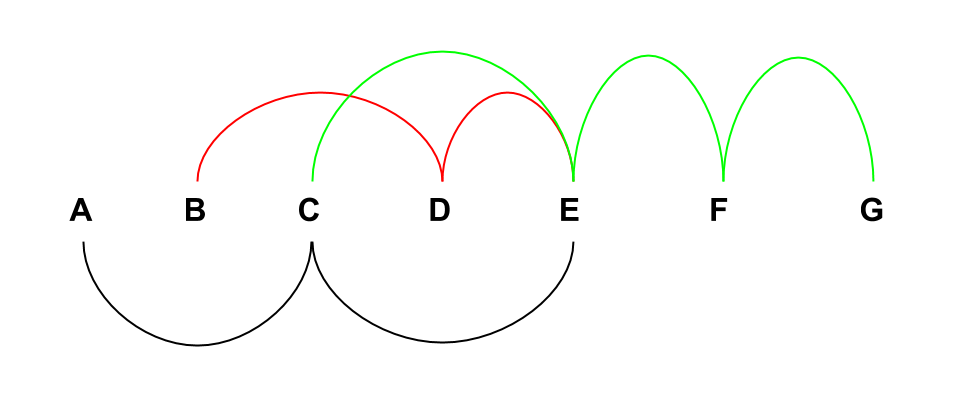
\includegraphics[height=2in]{examplePic_startingProblem.png}
\caption{Data Units with varying access requirements}
\end{figure}
Currently the total seek time is 11 units. Without redundancy, this is the optimal solution:\\
\begin{figure}[H]
\centering
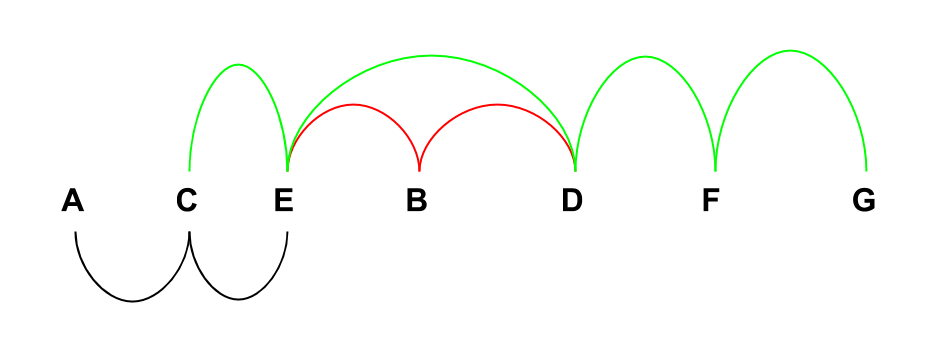
\includegraphics[height=2in]{examplePic_woRedundancy.png}
\caption{Optimal layout without redundancy}
\end{figure}
The seek time has been reduced to 9 units without using redundancy. With redundancy, this is the result:\\
\begin{figure}[H]
\centering
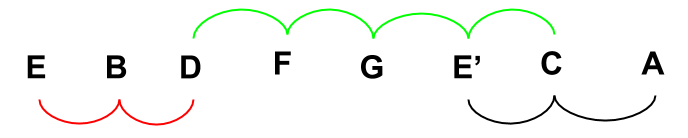
\includegraphics[height=2in]{examplePic_withRedundancy.png}
\caption{Optimal layout with redundancy}
\end{figure}
Here is an optimal layout with redundancy. The total seek time is now the minimum required which is 7 units. While a reduction from 9 to 7 units may not seem dramatic, when this result is scaled up to the hundreds of millions, this makes a big difference in seek time, as we saw in practice. 

\section*{Experimental Results}

**INSERT THE INFO FROM SHAN'S THESIS**

\section*{Conclusion and Future Work}

We have shown that we have a quadratic time algorithm with quadratic storage space for the Data Layout Problem. It achieves significant results analytically and experimentally. When walking through an extremely detailed 3D model, this algorithm can be used to ensure that the performance will not suffer. If we give the algorithm the proper access requirements with this 3D model, then the performance will be even better.\\
\\
This leads to a logical extension of this work. Since we have a good algorithm that takes over once we know the access requirements, we should figure out how to ensure there are good access requirements to begin with. One idea on how to ensure this is to check the usage history of an application and group data units together if they are accessed together with high probability. This could even be done dynamically in the sense that after a certain amount of usage and repeating on a regular basis, you recompute the optimal access requirements and then use that to recompute the optimal layout. 

\section*{Acknowledgments}

\newpage

\bibliographystyle{plain}
\bibliography{finalPaperRefs}

\newpage

\section*{Appendix}

\subsection*{Algorithm Summary}

\begin{verbatim}

Initialize AR heap and newCopy list
for each accessRequirement P's head node and tail node U:
     Set benefit to distance from U to next or previous node
     Let destination be spot with least number of overlapping access requirements
     For each access requirement T that also uses U
          See if T will be shorter by using new copy. Add T to oldCopyList if not.
          Add that to benefit if so
     Add benefit to heap
     If oldCopyList is empty then add U to newCopy list
while newCopy is not empty:
     take out random element and move the node
     Update AR heap and newCopy list
while there exists more space for redundancy:
     pop best element from heap
     copy the element U to its destination
     update affected access requirements
     update heap

\end{verbatim}
 

%\begin{figure}[H]
%\centering
%\includegraphics[height=4in]{prob1plot.jpg}
%\caption{Probability of Class Labels with decision boundaries marked}
%\end{figure}


\end{document}








